\begin{picture}(0,0)%
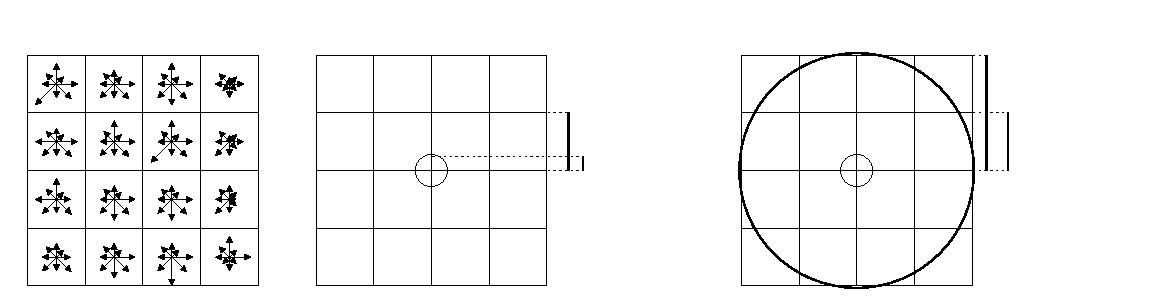
\includegraphics{doc/figures/sift-descr-easy-raw.ps}%
\end{picture}%
\setlength{\unitlength}{3035sp}%
%
\begingroup\makeatletter\ifx\SetFigFont\undefined%
\gdef\SetFigFont#1#2#3#4#5{%
  \reset@font\fontsize{#1}{#2pt}%
  \fontfamily{#3}\fontseries{#4}\fontshape{#5}%
  \selectfont}%
\fi\endgroup%
\begin{picture}(11747,2832)(-39,-1972)
\put(8701,689){\makebox(0,0)[b]{\smash{{\SetFigFont{9}{10.8}{\familydefault}{\mddefault}{\updefault}{\color[rgb]{0,0,0}Gaussian window}%
}}}}
\put(4276,689){\makebox(0,0)[b]{\smash{{\SetFigFont{9}{10.8}{\familydefault}{\mddefault}{\updefault}{\color[rgb]{0,0,0}magnification factor}%
}}}}
\put(6001,-736){\makebox(0,0)[lb]{\smash{{\SetFigFont{9}{10.8}{\familydefault}{\mddefault}{\updefault}{\color[rgb]{0,0,0}keypoint scale}%
}}}}
\put(5776,-286){\makebox(0,0)[lb]{\smash{{\SetFigFont{9}{10.8}{\familydefault}{\mddefault}{\updefault}{\color[rgb]{0,0,0}bin size}%
}}}}
\put(1276,689){\makebox(0,0)[b]{\smash{{\SetFigFont{9}{10.8}{\familydefault}{\mddefault}{\updefault}{\color[rgb]{0,0,0}Spatial histogram of gradients}%
}}}}
\put(10351,-736){\makebox(0,0)[lb]{\smash{{\SetFigFont{9}{10.8}{\familydefault}{\mddefault}{\updefault}{\color[rgb]{0,0,0}bin size}%
}}}}
\put(10201,314){\makebox(0,0)[lb]{\smash{{\SetFigFont{9}{10.8}{\familydefault}{\mddefault}{\updefault}{\color[rgb]{0,0,0}Gausian window}%
}}}}
\end{picture}%
